\chapter{gaNitadalilxruva kAvayx-dhavxni}\label{chap13}

\begin{wrapfigure}{r}{0.4\textwidth}
  \centering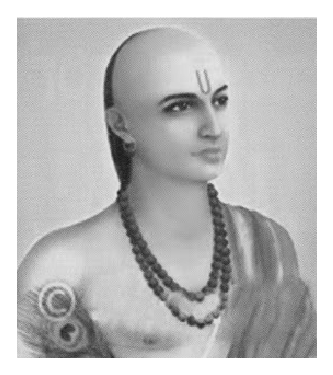
\includegraphics[scale=0.8]{src/figures/bhaskaracharya-II.eps}
  
  {\bf citarx~:~ BAsakxrAcAyaR}
    \end{wrapfigure}
    
BAratiVya gaNitada cariterxyalilx eraDaneya\break BAsakxrAcAyaRru atayxMta janapirxya vayxkitxgaLu.\- gaNita matutx KagoVLashAsatxrXgaLalilx ivara\break koDuge amUlayxvAdadudx. kirx.sha.\ $1150$ralilx tamamx $36$neya vayasisxnalilx ``sidAdhxMta shiroV\-maNi'' eMba garxMthavanunx saMsakxqqtadalilx racisidAdxre.

``sidAdhxMta shiroVmaNi'' eMbudu oMdu baqhatf garxMtha. adaralilx liVlAvati, biVjagaNitaM,\- garxhagaNitaM matutx goVlAdhAyxya eMba nAlukx BAgagaLive. ivugaLanunx nAlukx savxtaMtarx kaqtigaLeMdu parigaNisutAtxre.

sidAdhxMta shiroVmaNi eMba garxMthadalilx liVlAvati bahaLa parxsidadhxvAgide. liVlAvatiyanunx tiLidavaru maragaLalilxruva elegaLanunx heVLabahudu enunxtitxdadxraMte. kaSaTxkaravAda gaNitada samaseyxgaLanunx, kilxSaTxkara gaNita niyamagaLanunx atimanoVhara sholxVkagaLalilx balu sulaBa ``udAharaNegaLa mUlaka'' liVlAvati eMba garxMthadalilx vivarisidAdxre. idaralilx $277$ sholxVkagaLive.

\eject

idaralilxna bareha shirxV gaNeVshana pArxthaRneyiMda AraMBavAgutatxde. oMdoMdu sUtarxvanUnx parxshenxyanUnx padayxda rUpadalilx racisi kivige iMpAgiruvaMte ramaNiVyavAda vaqtatxgaLanunx Arisi, avugaLalilx giNi, haMsa, hAvu, navilu, maNi, mANikayx modalAdavugaLa vaNaRneyanunx tuMba citAtxkaSaRkavAgi magaLige boVdhisidAdxre. magaLa hesarU liVlAvatiyeV.

liVlAvati keVvala gaNitagarxMthavalalxde utatxmavAda kAvayxvU Agide. rasaBAva puSiTxgU upamA alaMkAragaLU citarxvicitarxvAda vaNaRnegaLU idaralilx tuMbive.

idara oMdu sholxVkadalilx tananx kavitA pwrxDhimeyanunx toVrisidAdxre.
\begin{center}
\begin{tabular}{l}
{\bf yeVSAM sujAti guNavagaR viBUtitAMgiV}\\
{\bf shudAdhxKila vayxvahaqtiH Kalu kaMThasakAtx |}\\
{\bf liVlAvatiVha sarasoVkitx mudAharaMtiV}\\
{\bf teVSAMsadeYva suKa saMpadupeYti vaqdidhxM ||}
\end{tabular}
\end{center}

I sholxVkavanunx eraDu athaRgaLanunx hoMduvaMte baredu BAsakxra tamamx kavitA pwrxDhimeyanunx toVrisidAdxre.

oMdu athaR: satukxladavaLAgiyU oLeLxya guNagaLiMdalU naDateyiMdalU kUDi, maqduBASaNavanunx mADatakakx lalanAmaNiyanunx paDediratakakx puruSanige yAvAgalU suKa saMpatutxgaLu vaqdidhxhoMdutAtx irutatxve.

matotxMdu athaR: jAti - BinanxrAshi, guNa - guNAkAra, vagaR - saMKeyxya vagaR, BinanxrAshigaLu, guNAkAra, vagaR muMtAda lekakxgaLiMda alaMkaqtavAgi tapipxlalxda gaNita vidhigaLiMda kUDi, sulaBavAda sheYliyalilx bareyalapxTiTxruva liVlAvati garxMthavanunx yAru kaMThapATha mADirutAtxroV (cenAnxgi tiLidukoMDirutAtxroV) avarige yAvAgalU suKa saMpatutxgaLu vaqdidhxyAgutatxve.



